\section{Network Architecture} \label{sec:netarc}


%=============================================================================%

The LSST Observatory is distributed over four sites: the Summit Site, the Base Site, the Archive Site, 
and the Project Headquarters. While the sites are geographically distributed, they are all functionally 
integrated. Dedicated high-bandwidth fiber optic lines connect the summit and base, with the others 
connected through secure shared networks. Control functions are distributed for operational efficiency 
and to provide robust, reliable, safe operation.

%=============================================================================%

The key driving requirements for the Mountain Summit to the Base Center communications are the 
bandwidth and reliability required to transfer the crosstalk-corrected image data for alert processing and 
the raw image data for forwarding to the Archive Center. Because this link closely follows the path of 
existing CTIO networks, LSST will manage and maintain this mission-critical link, providing the reliability 
and availability necessary to run the combined Mountain-Base infrastructure as a single component of 
the LSST system.

%=============================================================================%

The complete network infrastructure for the LSST has been designed based on existing hardware 
solutions. The details of the network design are in LSE-78. The network spans several distinct locations 
as shown in Figure~\ref{fig:global_netarc}.

%=============================================================================%

\begin{figure}
\begin{center}
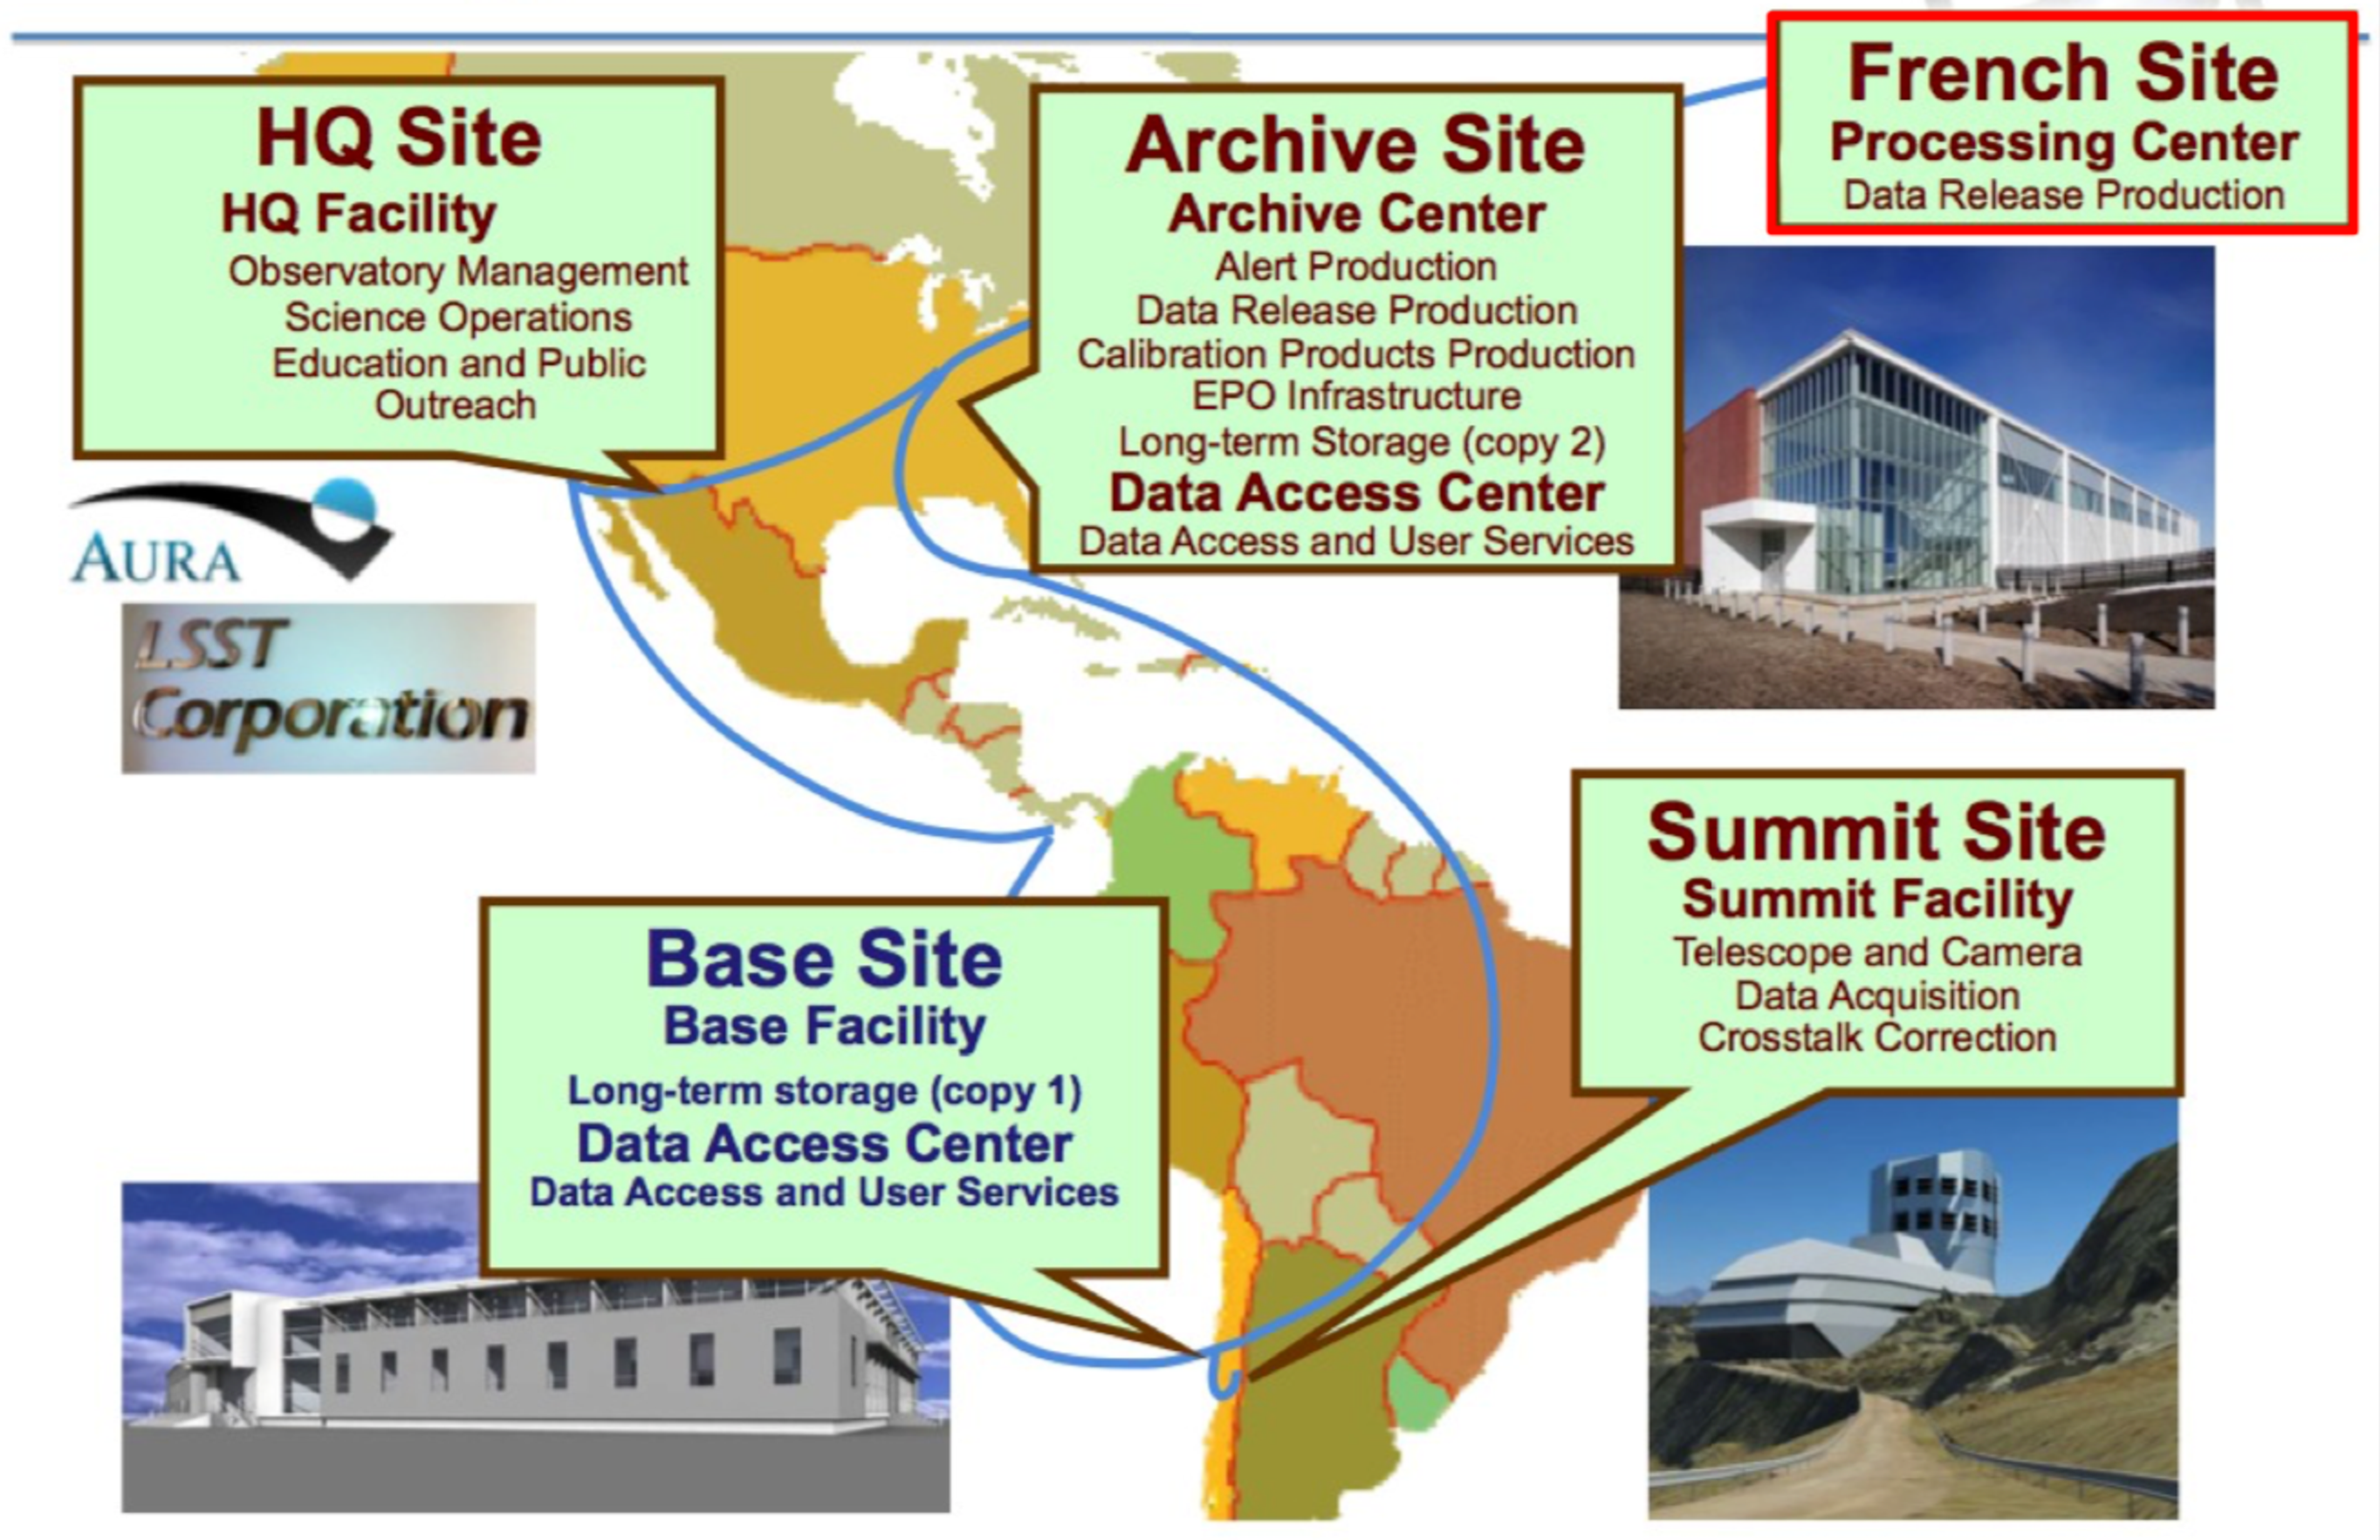
\includegraphics[width=0.6\textwidth]{global_netarc}
\caption{Global network architecture diagram. \label{fig:global_netarc}}
\end{center}
\end{figure}

%=============================================================================%

Figure~\ref{fig:local_netarc} shows the detailed implementation of the summit networking system. The 
central data center switches, Cisco 5548, will be completely redundant and serve the whole of the 
summit network and computer systems integrating the Telescope and Camera subsystems. 
Automatic failover will occur in the event of a switch failure. This model switch is Cisco?s latest 
technology with low latency and 192 Tb/s switching fabric. The Cisco 5528 access switches use dual
ported uplinks in a mesh configuration and connected by fabric extenders to offer 10 Gb/s bandwidth 
throughout the summit. Up to 16 ports can be aggregated to form a maximum of 1.6 Tb/s channel. 
The goal is to interconnect all network devices with fiber cable wherever possible and so optimize 
transmission with SPF connectors. The diagram indicates in each network box where that equipment 
will reside, i.e. cr = computer room, tu = telescope utility area, do = dome, etc.

%=============================================================================%

\begin{figure}
\begin{center}
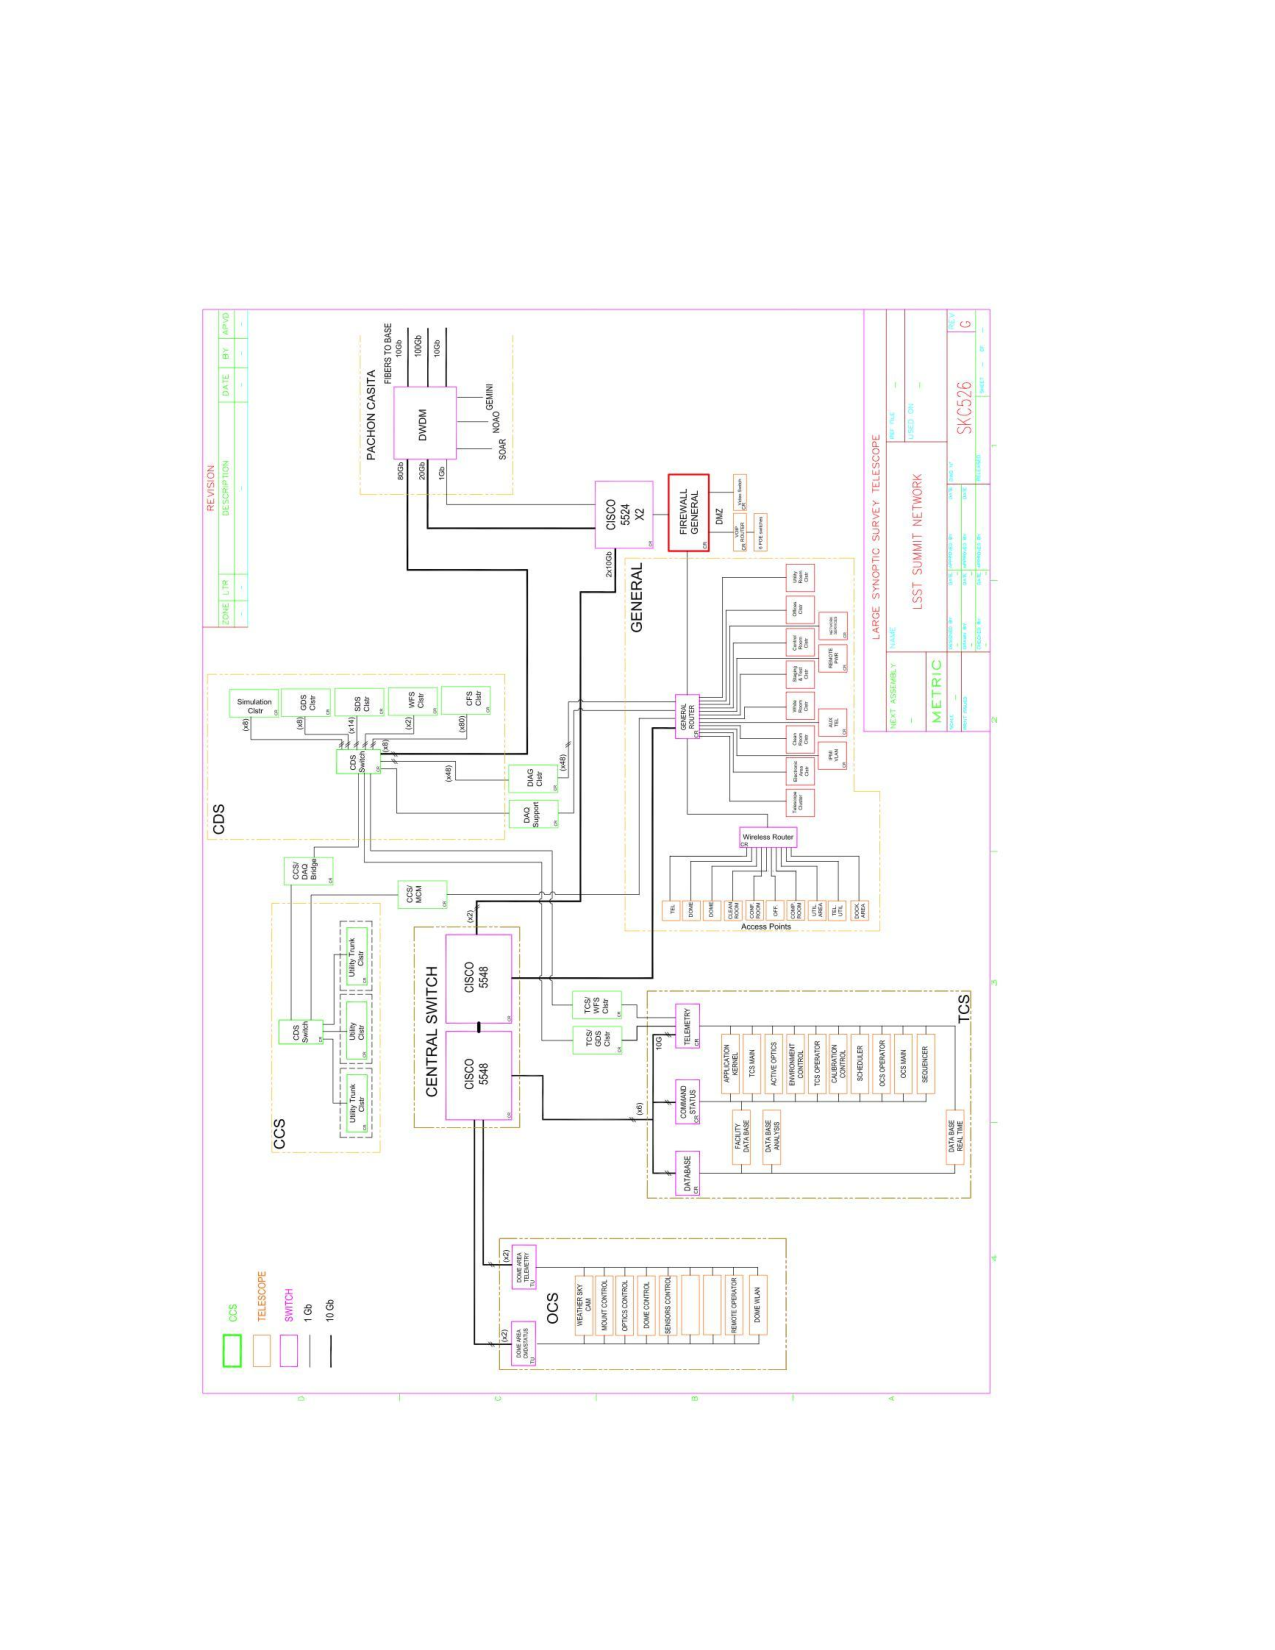
\includegraphics[width=0.5\textwidth,angle=270]{local_netarc}
\caption{Summit network system. \label{fig:local_netarc}}
\end{center}
\end{figure}

%=============================================================================%
